\section{问题2：第二检测点的选择与候选区域}

\subsection{任务与“较好”的含义}

已知一个全向干扰源在检测点 $s$ 处的示向度 $\hat\theta$，真位置 $g$ 与接收半径 $r_i$ 均未知。需要给出第二个检测点 $q$ 的选择策略，以及 $q$ 所在的候选区域。题面没有指定“较好”的数值指标。若把未知真值上的期望定位误差当作目标，策略在线不可计算；若只最大化两射线夹角，则忽略 $r_i$ 可能使第二点收不到信号。传感器布置理论指出，基线与夹角共同决定几何精度因子\upcite{zhao_2013_placement}\upcite{moreno_2013_placement}，主动采集方位时还要计入行走代价\upcite{bayram_2016_bearing}。本文把“较好”落实为：在保证第二点对 $F_1$ 外包络尽可能可观测的前提下，使最坏后验包围半径的排序估计 $J(q)$ 尽量小，并以行走时间作为同 $J$ 时的次级键。该指标用于候选集内部排序，不是清除证书。

“较好”还必须服从接口约束。第二点仍只能得到三值反馈，不能假设一定收到示向度；同一点重复测量不是新样本，因而候选集里不应把 $s$ 附近的加密点当成独立测向。机器狗坐标分量绝对值不得超过 $2\times 10^6\,\mathrm{m}$，越界点直接丢弃。问题2只讨论一个全向源，不涉及频道判空，也不把 $J(q)\le 20$ 写成现场可清。

验证分三级，正确性是硬门。
真值必须落在所声称的外包与后验内；“保证可观测”必须对所声称的集合成立；“确定可清”仅当后验包围半径不超过 $20\,\mathrm{m}$。
这三级失败不得解释成定位效果差，而应标成模型或实现错误。
鲁棒性检查示向度微扰、近区 $5\,\mathrm{m}$ 边界、接收半径取端点 $1000$ 与 $1500$，以及核心圆边界。
无信号支不得写成 $F_1$ 挖掉以 $q$ 为心的 $1000\,\mathrm{m}$ 开球，因为外包已经用 $1500\,\mathrm{m}$ 切线放大，挖球会把仍可能有源的点删掉。
效率只比较候选规模与相对加密参考集的 $J$ 间隙，不证明连续全局最优。
建议容差：距离 $10^{-8}$ 至 $10^{-6}\,\mathrm{m}$，角度 $10^{-10}$ 至 $10^{-6}$ 度，核心圆 $10^{-6}\,\mathrm{m}$，未裁剪扇形 $\rho_1\le 750.114+8\,\mathrm{m}$ 以容纳外包切线余量。
开发集种子为分层 $20$ 例，编号 $12000$ 至 $12019$，独立单元是第一次示向度加第二次测量；第二点误差由种子与量化坐标绑定，不按调用序号重抽。
频率不是检测概率。一级失败则不写“更优”对比。

\subsection{第一点后的可行外包}

单次 $\mathtt{direction}$ 给出前向闭楔形。源还落在 $\Omega$ 内，且与 $s$ 的距离不超过 $r_i\le 1500$。$5\,\mathrm{m}$ 近区在第一点并未触发 $\mathtt{near}$，严格地说 $F_1$ 应挖去以 $s$ 为心的 $5\,\mathrm{m}$ 开圆，但挖洞使集合非凸，对第二点排序没有帮助。本文用凸外包
\begin{equation}
\widetilde F_1=\mathrm{Wedge}(s,\hat\theta,\varepsilon)\;\cap\;\Omega_{\mathrm{out}}\;\cap\;\overline B(s,1500),
\end{equation}
其中 $\Omega_{\mathrm{out}}$ 是 $\Omega$ 的外切正多边形（实现取 $48$ 条切线），$\overline B(s,1500)$ 同样用切线外包。$\widetilde F_1$ 包含真 $F_1$，顶点由半平面枚举得到。最小包围圆圆心记为 $c_1$，半径记为 $\rho_1$。演示数据在 $s=(0,0)$、$\hat\theta=0^\circ$ 时给出 $\rho_1\approx 750.2285094687356\,\mathrm{m}$，$c_1\approx(750.2285094687359,0)$。

理论扇半径来自几何观察：最大接收半径 $1500\,\mathrm{m}$ 的前向 $2\varepsilon$ 楔形，其最小包围圆半径为
\begin{equation}
\rho_{\mathrm{th}}=\frac{r_{\max}}{2\cos\varepsilon}\approx 750.1142460329307\,\mathrm{m}.
\end{equation}
$\rho_1$ 与 $\rho_{\mathrm{th}}$ 接近而略大，因为 $\Omega$ 的切线外包与楔形相交后并不恰好是理想扇。核心可观测半径取
\begin{equation}
R_{\mathrm{core}}=\max\{r_{\min}-\rho_1,\,1\}\approx 249.77149053126436\,\mathrm{m}.
\end{equation}
落在 $\overline B(c_1,R_{\mathrm{core}})$ 内的第二点，对 $\widetilde F_1$ 上每一点的距离不超过 $1000\,\mathrm{m}$，从而在“外包被 $1000\,\mathrm{m}$ 控制”的意义下对第一层近似可观测。这仍是充分条件的保守形式，不是现场保证：真 $r_i$ 可能小于 $1000+\rho_1$，核心圆外的点仍可能收到信号，核心圆内的点在外包被放大时也可能对某些边界点不可测。

\begin{figure}[H]
\centering
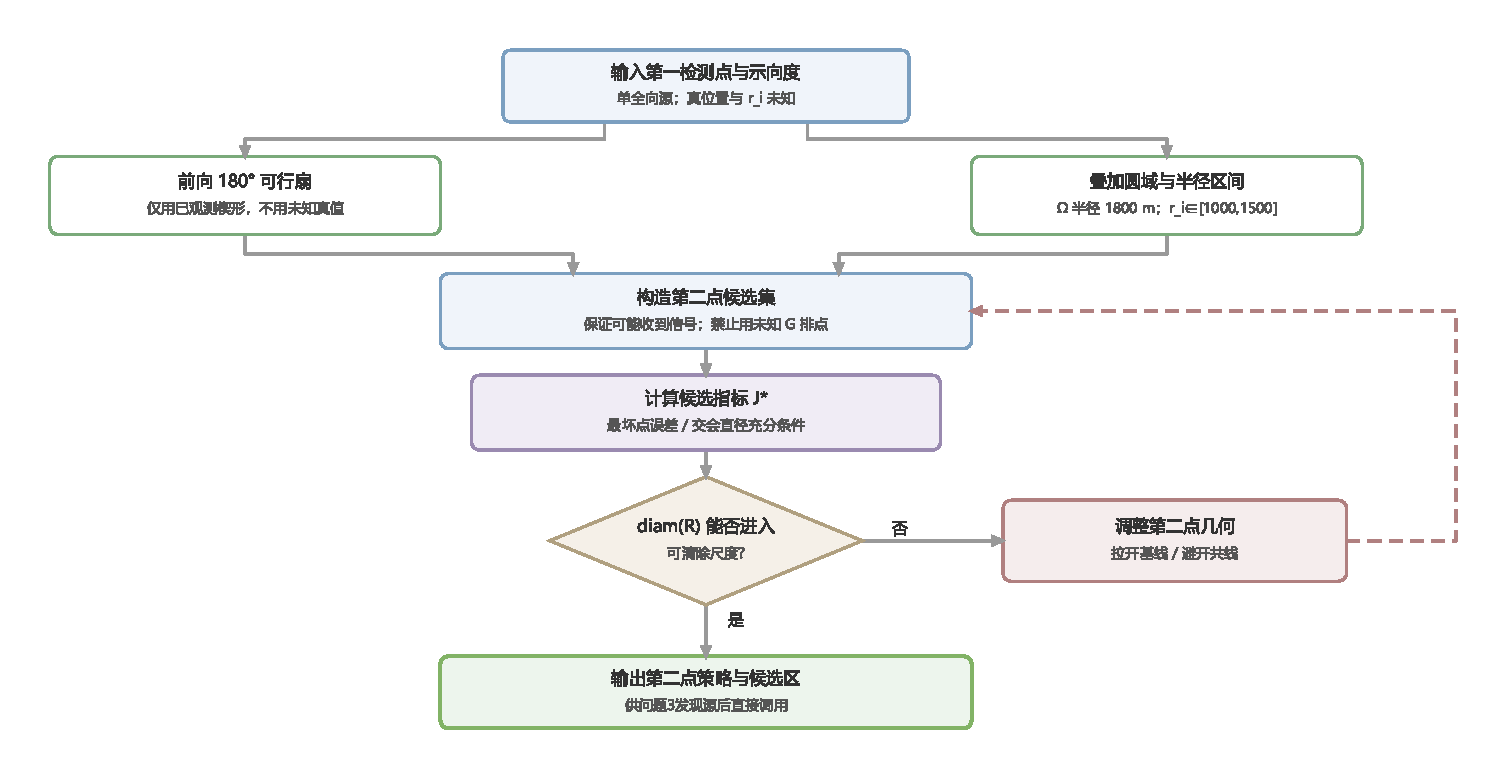
\includegraphics[width=0.82\textwidth,height=0.52\textheight,keepaspectratio]{../figures/fig_flow_q2.pdf}
\caption{问题2第二点求解流程}
\label{fig:flow_q2}
\end{figure}

流程先构造 $\widetilde F_1$ 与核心圆，再在核心、保证环与探索环上采样。
用 $J(q)$ 排序后做局部加密。
输出声明为候选集推荐，避免把 $q^\ast$ 写成唯一现场第二点。
分层的目的是把尽量可观测与尽量压缩角向不确定性分开：前者优先落在核心圆，后者才允许走到保证环甚至探索环。
行走时间只作为同 $J$ 时的次级键，防止策略为了零点几米的排序差而绕远。
正确性是硬门：真值必须落在所声称的外包与后验内，保证可观测必须对所声称的集合成立，确定可清仅当后验包围半径不超过 $20\,\mathrm{m}$。
这三级失败不得解释成定位效果差，而应标成模型或实现错误。

\subsection{排序指标 $J(q)$}

第二点 $q$ 的反馈仍是三值。
对 $\widetilde F_1$ 边界采样点集合 $S$，按反馈分支估计后验包围半径。
若 $\|x-q\|\le 5$ 的采样非空，该支取 $\min\{5,\rho(S_{\mathrm{near}})\}$。
若存在采样满足 $\|x-q\|>\max\{1000,\|x-s\|\}$，该支取这些点的包围半径，对应可能的 $\mathtt{no\_signal}$。
对其余点按 $2^\circ$ 网格扫描可能的示向度，每条示向度对应 $\pm 1^\circ$ 内的采样子集，取最坏包围半径。
$J(q)$ 定义为各支的最大值。
$J$ 是外包络上的排序估计，边界采样不能穷尽连续集合，因此即使 $J(q)\le 20$ 也不能签发清除证书。

候选点分四层。A 层在核心圆内按极环采样；B 层在核心外但满足“对全部采样 $\widetilde F_1$ 点，到 $q$ 的距离不超过 $\max\{1000,\|x-s\|\}$”的保证环；C 层是其余探索环；另把 $s$ 自身列入对照。对 $J$ 有限的候选按 $(J,$ 行走时间 $)$ 字典序排列，取前三名做步长 $\max\{5,R_{\mathrm{core}}/16\}$ 的网格加密。演示数据共 $191$ 个候选，层计数 A $65$、C $19$、B $31$、$s$ $1$、refine $75$，最优
\begin{equation}
q^\ast\approx(719.0070731523278,\,634.1607723730604),\qquad J^\ast\approx 43.0312146778083\,\mathrm{m},
\end{equation}
行走时间约 $191.74264590433432\,\mathrm{s}$。$J^\ast>20$，说明即便按该推荐布点，外包最坏半径仍大于光学半径，第二点之后通常还需要累计测向或光学网格，而不能宣称一次交会即可清除。把 $s$ 列入对照是为了防止策略退化成“原地再测一次”：同点误差不刷新，原地测量只会支付时间。

\subsection{候选区域}

候选区域不是一个随意画出的椭圆，而是上述分层采样的几何载体。
核心圆 $\overline B(c_1,R_{\mathrm{core}})$ 给出尽量可观测的内区；保证环给出对第一点外包仍不丢信号的扩大带；探索环允许为了压缩角向不确定性而牺牲部分可观测性。
机器狗坐标仍受 $|q_x|,|q_y|\le 2\times 10^6$ 约束，实现中越界点直接丢弃。
策略上优先 A 层，A 层 $J$ 接近时再看行走时间；仅当核心过小或 $J$ 平台时进入 B、C。
问题3发现源后的第二测点模块调用同一套几何，但在覆盖巡回途中会改用局部横向偏移，以免为了理论 $q^\ast$ 而破坏七点巡回：沿示向度前进约 $500\,\mathrm{m}$ 并横向偏移 $150\,\mathrm{m}$；若当前位姿已经满足沿向 $\ge 200\,\mathrm{m}$ 且横向 $\ge 80\,\mathrm{m}$，则就地作为第二点。
演示数据共 $191$ 个候选，层计数核心 $65$、保证环 $31$、探索环 $19$、对照点 $1$、加密 $75$，说明加密层才把推荐点从粗网格推到 $q^\ast$。
开发集候选点数中位数只有 $62$，因为开发集不含演示那一层局部加密，不能把 $191$ 写成现场固定规模。

\begin{figure}[H]
\centering
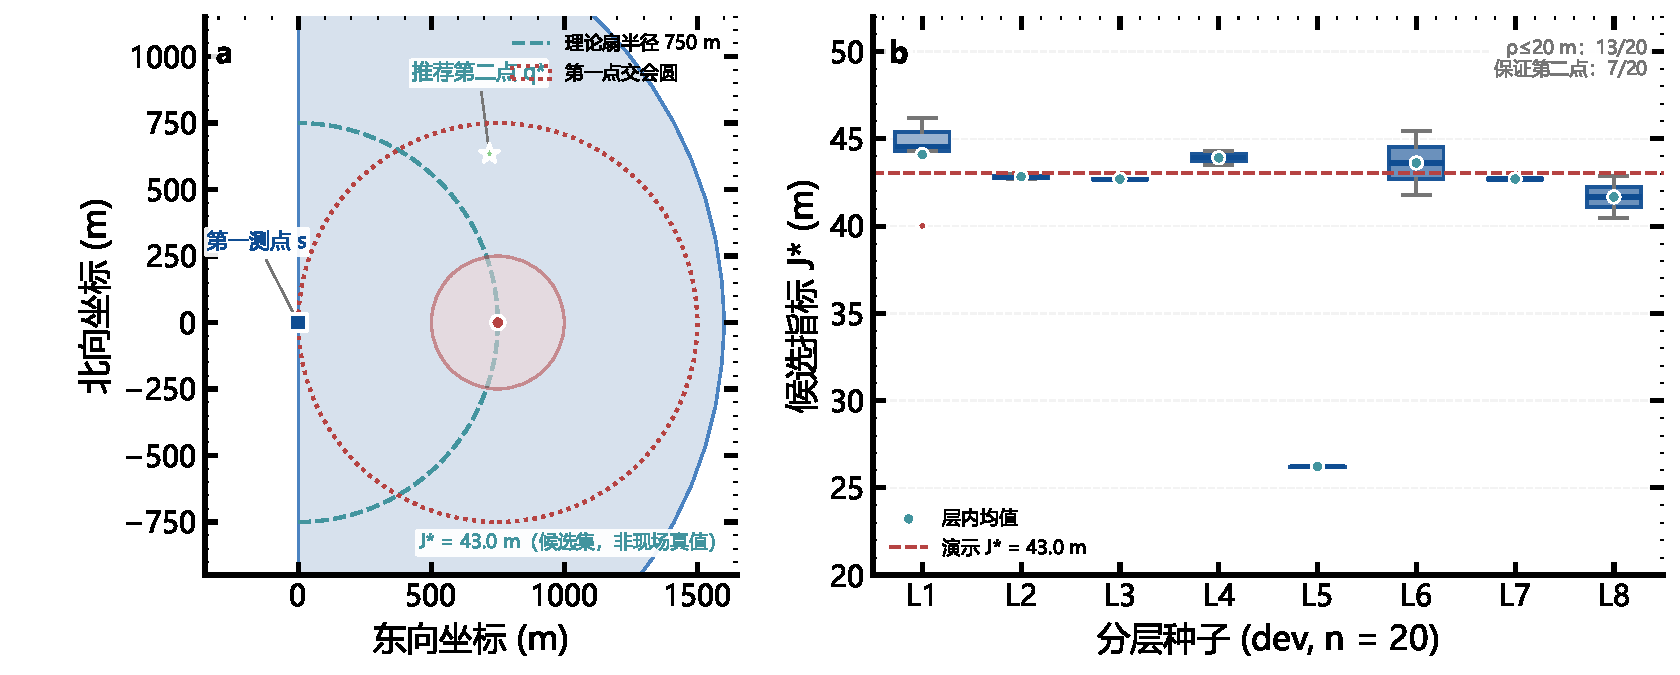
\includegraphics[width=0.95\textwidth]{../figures/fig_q2_candidate.pdf}
\caption{第二测点几何与$J$分布}
\label{fig:q2_candidate}
\end{figure}

左面板画出前向扇形示意、理论半径约 $750.1142460329307\,\mathrm{m}$ 以及推荐点 $q^\ast$。
右面板是分层种子开发集 $n=20$ 上 $J^\ast$ 的分布。
开发集上 $J^\ast$ 的中位数 $42.75989\,\mathrm{m}$，$90\%$ 分位 $45.40667\,\mathrm{m}$，$95\%$ 分位 $45.48670\,\mathrm{m}$，最大值 $46.20539\,\mathrm{m}$，全部明显高于 $20\,\mathrm{m}$。
同一批种子里，用真值后验包围半径不超过 $20\,\mathrm{m}$ 的比例为 $13/20$，满足保证第二点条件的比例为 $7/20$。
这些比例是生成器下的经验频率，不是竞赛概率，也不是清除证书率。
一级不变量在二十个种子上全部通过：真值落入第一层外包，未签发虚假清除证书，失败种子列表为空。
二十次第二反馈均为 $\mathtt{direction}$，没有 $\mathtt{near}$ 或 $\mathtt{no\_signal}$；该生成器把第一点放在可测位置，因而不能外推到任意第一点都收得到信号。
行走时间中位数约 $202.8318\,\mathrm{s}$，与演示的 $191.74264590433432\,\mathrm{s}$ 同量级。
$J(q^\ast)$ 相对在 $c_1$ 处直接取值的均值差为 $-271.014$，说明排序确实把候选从包围圆心推开，而不是退化为走到 $c_1$。

\subsection{小结}

问题2给出可计算的第二点策略：用凸外包代替未知 $F_1$，用 $J(q)$ 在分层候选上排序，并用理论扇半径标定核心尺度。首先构造 $\widetilde F_1$ 与 $\rho_{\mathrm{th}}$；再定义核心圆与三层候选；接着用边界采样估计各反馈分支的最坏后验半径；最后在演示与开发集上核对 $J^\ast$ 始终大于 $20\,\mathrm{m}$。演示推荐点的 $J^\ast\approx 43.03\,\mathrm{m}$ 明确大于光学半径，因此该问的交付是“候选区域与排序”，而不是“保证一次测向后即可光学清除”。后文在线策略把这一模块降级为发现后的局部测向，完备性仍交给覆盖证书与光学网格。开发集 $n=20$ 只用于不变量与经验频率，不得写入正式测试表。

开发集按方位分成八层，种子编号 $12000$ 至 $12019$，独立单元是第一次示向度加第二次测量。
一级不变量失败计数全为零：真值落入第一层外包与第二层后验的失败为 $0$，外包包含真源失败为 $0$，核心层虚假保证为 $0$，虚假清除证书为 $0$，同半径约束违反为 $0$，失败种子列表为空。
二级统计里真值后验半径中位数 $16.041006961792853\,\mathrm{m}$ 低于光学半径，但 $90\%$ 分位 $33.98821640813881\,\mathrm{m}$、$95\%$ 分位 $34.52792979405194\,\mathrm{m}$、最大值 $44.23995719791731\,\mathrm{m}$ 仍高于 $20\,\mathrm{m}$，与 $13/20$ 的经验频率一致：第二点有时已经足够小，有时仍需要第三次测向或光学网格。
保证第二点比例只有 $7/20$，说明核心圆并不是多数场景下的现场保证，只能作为排序层的几何载体。
无信号比例为 $0/20$，第七层两例同样没有无信号，该生成器不能用来讨论第二点收不到射频的情形。
分层内部 $J^\ast$ 中位数：第一层五例 $44.579097685173345\,\mathrm{m}$，第二层三例 $42.79810125316518\,\mathrm{m}$，第三层两例 $42.69319615796\,\mathrm{m}$，第四层两例 $43.911666500687936\,\mathrm{m}$，第五层两例 $26.221913542405897\,\mathrm{m}$，第六层两例 $43.62023178395506\,\mathrm{m}$，第七层两例 $42.69840923489445\,\mathrm{m}$，第八层两例 $41.6697527153196\,\mathrm{m}$。
第五层较低并不改变全体高于 $20\,\mathrm{m}$ 的结论，也不能把某一层写成“已经可清”。
相对加密参考集的 $J$ 间隙中位数 $0.054647539414797316\,\mathrm{m}$，$90\%$ 分位 $0.29573075412744654\,\mathrm{m}$，$95\%$ 分位 $0.30476672767477625\,\mathrm{m}$，最大 $0.3478972173578117\,\mathrm{m}$，只说明分层候选相对加密网格没有大幅变差，不证明连续全局最优。
示向度微扰的 $J$ 抖动在该批开发集上样本数为 $0$，正文不把空统计写成稳定性结论。
CPU 中位数约 $0.235078\,\mathrm{s}$，$90\%$ 分位约 $0.263876\,\mathrm{s}$，最大约 $0.268550\,\mathrm{s}$，墙钟不是本题指标，只说明该模块可以嵌进在线循环而不单独吃掉 $1200\,\mathrm{s}$ 程序时限。
候选点数中位数 $62$，十分位上沿 $62.1$，$95\%$ 分位 $63$，最大 $63$，与演示的 $191$ 不同，因为演示含局部加密层。
行走时间中位数 $202.8318011676986\,\mathrm{s}$，$90\%$ 分位 $214.37254386177045\,\mathrm{s}$，$95\%$ 分位 $221.52990439172441\,\mathrm{s}$，最大 $270.4007286633272\,\mathrm{s}$。
建议容差为距离 $10^{-8}$ 至 $10^{-6}\,\mathrm{m}$，角度 $10^{-10}$ 至 $10^{-6}$ 度，未裁剪扇形 $\rho_1\le 750.114+8\,\mathrm{m}$ 以容纳外包切线余量。
声明限制为自建分层场景，不是竞赛概率，也不是连续全局最优。
留出集 $22000$ 至 $22099$ 共一百例在冻结后只报一次，正文不把尚未写入结果汇总的留出均值写成新实验。
